\documentclass[conference]{IEEEtran}

% correct bad hyphenation here
\hyphenation{op-tical net-works semi-conduc-tor}
\usepackage{amsmath}
\usepackage{comment}
\usepackage{graphicx}
%\usepackage{cases}
%\usepackage{subeqnarray}

\usepackage{multicol}
\usepackage{lipsum}
\usepackage{mathtools}
\usepackage{cuted}

\usepackage{extpfeil}
\usepackage{mathpartir}
\usepackage[mathscr]{eucal}

\usepackage{hyperref}
\usepackage{cleveref}
\crefformat{section}{\S#2#1#3} % see manual of cleveref, section 8.2.1
\crefformat{subsection}{\S#2#1#3}
\crefformat{subsubsection}{\S#2#1#3}

\usepackage{algorithm}
\usepackage{algorithmicx}
\usepackage{algpseudocode}
\renewcommand{\algorithmicrequire}{\textbf{Input:}}
\renewcommand{\algorithmicensure}{\textbf{Output:}}

\usepackage{color}
\usepackage{xcolor}
\newcommand{\todo}[1]{\textcolor{red}{[TODO: #1]}}


\begin{document}
%
% paper title
% Titles are generally capitalized except for words such as a, an, and, as,
% at, but, by, for, in, nor, of, on, or, the, to and up, which are usually
% not capitalized unless they are the first or last word of the title.
% Linebreaks \\ can be used within to get better formatting as desired.
% Do not put math or special symbols in the title.
\title{Multiple Object Tracking with DeepSORT, LSTM, and More Kalman Filters}
%
%
% author names and IEEE memberships
% note positions of commas and nonbreaking spaces ( ~ ) LaTeX will not break
% a structure at a ~ so this keeps an author's name from being broken across
% two lines.
% use \thanks{} to gain access to the first footnote area
% a separate \thanks must be used for each paragraph as LaTeX2e's \thanks
% was not built to handle multiple paragraphs
%

\author{
    Shangning Xu,
    Zhongye Wang,
    Xinyu Zhan
}

% The paper headers
% \markboth{Journal of \LaTeX\ Class Files,~Vol.~13, No.~9, September~2014}%
% {Shell \MakeLowercase{\textit{et al.}}: Bare Demo of IEEEtran.cls for Journals}
% The only time the second header will appear is for the odd numbered pages
% after the title page when using the twoside option.
%
% *** Note that you probably will NOT want to include the author's ***
% *** name in the headers of peer review papers.                   ***
% You can use \ifCLASSOPTIONpeerreview for conditional compilation here if
% you desire.


% make the title area
\maketitle

% As a general rule, do not put math, special symbols or citations
% in the abstract or keywords.
% \begin{abstract}
% The abstract goes here.
% \end{abstract}

% Note that keywords are not normally used for peerreview papers.
% \begin{IEEEkeywords}
% IEEEtran, journal, \LaTeX, paper, template.
% \end{IEEEkeywords}


\IEEEpeerreviewmaketitle

% \todo{From the project guideline: In the FIRST PARAGAPH of your final project report, please CLEARLY summarize which evaluation criteria your work is applicable to, for example, 1. Baseline, 2. Good, 3. Excellent. Meanwhile, please clearly present the supporting points why your work is applicable to such criteria, for example, novel  ideas, novel insights, performance gains, etc. If your improvement is small, it is not okay to overclaim contributions with better criteria.}

\section{Introduction}

\begin{quote}
    \textbf{Note:} It is advisable to read \texttt{README.md} first.
\end{quote}

We have aimed at achieving the excellent work by using more Kalman filters in more interesting ways.
However, we did not achieve all goals we have planned, so we are not sure our work is counted as good or excellent, but we list our achievement in all criteria below.
\begin{itemize}
    \item \textbf{Baseline:} We successfully get the DeepSORT code running, and generate the MOT metrics evaluation on the tracking results of MOT16 dataset. We use the DeepSORT code to generate tracking result of our own video, and we implement a real-time tracking application based on YOLO detections and DeepSORT.
    \item \textbf{Good:} We use YOLO \cite{redmon2016you}\cite{yolov3} to generate better detections and feed them to the DeepSORT framework. We explore the idea of using CNN-LSTM to approach the tracking problem, but do not have enough resources to implement the idea and run the training. We use deep Hungarian network \cite{xu2019deepmot} to replace the matching process in the DeepSORT. But they do not improve very much from the DeepSORT and we give some analysis of the results.
    \item \textbf{Excellent:} We extend the state representation of an object with the higher-order derivatives of its spatial coordinates and use Kalman filter to track those information for better translation prediction. We achieve 1\% improvement in IDF1 with slight sacrifices of MOTA. We attempt to apply Kalman filtering to the deep feature as well, but do not have enough time to implement the idea.
\end{itemize}

Per the licensing requirement of GPLv3, which is used by the implementation of Deep SORT and YOLOv3, our work is open-source on GitHub\footnote{Link: \url{https://github.com/BruceZoom/EI339-ProjectMOT}} throughout development.

\section{Understanding Deep SORT}

In this section, we give an overview of the implementation\footnote{Link: \url{https://github.com/nwojke/deep_sort}} by Nicolai and Alex \cite{Wojke2018deep} (referred to as ``their implementation'' in this section), on which our experiments in later sections are based.

Our presentation of the implementation is based on the following use case: the user has downloaded MOT16 \cite{milan2016mot16} dataset and wish to visualize Deep SORT's tracking performance on the dataset, by identifying people and tagging them by IDs. We shall explain various components associated with this use case.

\subsection{A High-Level View}

The entry point for this use case is the \texttt{run} function in the file \texttt{deep\_sort\_app.py}. The \texttt{run} function constructs an object of the class \texttt{Tracker}, which has a list of ``tracks'' (objects being tracked), represented by the class \texttt{Track}. Then the function \texttt{frame\_callback} is defined that accepts a \texttt{Visualization} object and a frame index as its parameters. The \texttt{Visualization} object contains an \texttt{ImageViewer} object that handles image display and drawing (like drawing bounding boxes).

On a fixed time interval, the \texttt{frame\_callback} function is called. \texttt{frame\_callback} reads the frame, the detections in \texttt{det.txt} (provided by MOT16) and pre-computed feature descriptors for each detection. Each detection is a bounding box in a frame. Then it calls the \texttt{predict} and \texttt{update} method of the \texttt{Tracker} object to perform matching and update the estimations of tracks' states. Confirmed detections are drawn on the frame and the frame is passed to the \texttt{Visualization} object (and in turn \texttt{ImageViewer}). Based on the keyboard input, the \texttt{ImageViewer} either pauses the video playback, steps through each frame, or exits.

\subsection{Generating Feature Descriptors}

It should be noted that, despite the word ``online'' in the name ``Deep SORT'', their implementation requires pre-computed feature descriptors for each detection. The file \texttt{generate\_detections.py} in the directory \texttt{tools} reads the detection file and uses a CNN (architecture given in \cite{Wojke2018deep}) to compute feature descriptors.

\subsection{Kalman Filter}

Only one \texttt{Tracker} object is created throughout execution. In the method \texttt{Tracker.predict}, each \texttt{Track} object's \texttt{predict} in \texttt{Tracker} method is invoked and passed a \texttt{KalmanFilter} object. \texttt{KalmanFilter} also has methods \texttt{predict} and \texttt{update} that take the state and the state error covariance as input. \texttt{update} additionally accepts a measurement as input.

Recall that the state vector for each track is
\[
    s = [u, v, \gamma, h, \dot{x}, \dot{y}, \dot{\gamma}, \dot{h}].
\]
\texttt{predict} and \texttt{update} implements the \texttt{predict} and \texttt{update} steps of a Kalman filter, respectively. We note the initial values for some parameters below that are otherwise omitted from \cite{Wojke2018deep}. The state-transition equation is
\[
    s_{k + 1} = Fs_k + w_k
\]
where $F$ is the state-transition matrix given by
\[
    F = \begin{bmatrix}
        I_4 & I_4\\
        \mathcal{O} & I_4
    \end{bmatrix}
\]
and $w_k \sim N(0, Q)$ is the noise, where
\[
    Q = \mathrm{diag}([\frac{h_k^2}{400}, \frac{h_k^2}{400}, 10^{-4}, \frac{h_k^2}{400}, \frac{h_k^2}{160^2}, \frac{h_k^2}{160^2}, 10^{-10}, \frac{h_k^2}{160^2}]).
\]

The measurement model is
\[
    z_k = Hs_k + v_k
\]
where $v_k \sim N(0, R)$ is the measurement noise and
\[
    R = \mathrm{diag}([\frac{h_k^2}{400}, \frac{h_k^2}{400}, 10^{-2}, \frac{h_k^2}{400}]).
\]

Exact formulas for prediction and update are omitted for brevity.

\subsection{Matching}

\texttt{Tracker.update} accepts a list of detections as input and when called, calls \texttt{Tracker.\_match} to solve the matching problem. \texttt{\_match} calls the function \texttt{matching\_cascade} in the file \texttt{linear\_assignment.py}, which uses the algorithm specified in Algorithm~\ref{alg:matching-cascade}. Unmatched tracks and detections are further matched with IOU.

\begin{algorithm}[t]
    \caption{Matching cascade, from \cite{Wojke2018deep}}
    \label{alg:matching-cascade}
    \begin{algorithmic}[1]
        \Statex \textbf{Input:} Track indices $\mathcal{T} = \{1, \dots, N\}$, Detection indices $\mathcal{D} = \{1, \dots, M\}$, Maximum age $A_\textrm{max}$
        \State Compute cost matrix $C = [c_{i,j}]$
        \State Compute gate matrix $B = [b_{i,j}]$
        \State Initialize set of matches $\mathcal{M} \gets \emptyset$
        \State Initialize set of unmatched detections $\mathcal{U} \gets \mathcal{D}$
        \For{$n \gets 1$ \textbf{to} $A_\textrm{max}$}
            \State Select tracks by age $\mathcal{T}_n \gets \{i \in \mathcal{T} | a_i = n\}$
            \State $[x_{i,j}] \gets \mathrm{min\_cost\_matching}(\mathcal{C}, \mathcal{T}_n, \mathcal{U})$
            \State $\mathcal{M} \gets \mathcal{M} \cup \{(i, j) | b_{i,j} \cdot x_{i,j} > 0\}$
            \State $\mathcal{U} \gets \mathcal{U} \setminus \{j | \sum_i b_{i,j} \cdot x_{i,j} > 0\}$
        \EndFor
        \State \Return $\mathcal{M}, \mathcal{U}$
    \end{algorithmic}
\end{algorithm}

\texttt{\_match} returns matches, unmatched tracks and unmatched detections. Unmatched tracks are marked as ``missed'' with the method \texttt{Track.mark\_missed}. Unmatched detections are used to initiate new tracks.

Table~\ref{tab:eval-deepsort} shows the baseline performance of the DeepSORT.

\begin{table}[h]
    \caption{Evaluation Result of the DeepSORT}
    \label{tab:eval-deepsort}
    \begin{tabular}{ccccccccc}
        \hline
        & MOTA & IDF1 & MT & ML & FP & FN & IDs\\\hline
        MOT16-02 & 34.2\% & 43.7\% & 8 & 12 & 2500 & 9148 & 89\\
        MOT16-13 & 60.5\% & 62.8\% & 53 & 11 & 1450 & 2877 & 197\\
        MOT16-09 & 65.6\% & 61.5\% & 12 & 1 & 172 & 1611 & 28\\
        MOT16-11 & 68.1\% & 64.7\% & 21 & 11 & 426 & 2473 & 32\\
        MOT16-05 & 54.0\% & 62.1\% & 26 & 28 & 410 & 2683 & 46\\
        MOT16-10 & 56.3\% & 56.6\% & 22 & 2 & 1940 & 3312 & 133\\
        MOT16-04 & 58.6\% & 71.1\% & 41 & 18 & 5327 & 14311 & 52\\
        OVERALL & 55.4\% & 62.9\% & 183 & 83 & 12225 & 36415 & 577\\\hline
\end{tabular}
\end{table}

\section{Other Existing Advanced Techniques}
Despite of deep cosine features and multi-stage matching, there have been other more recent works on solving the multiple object tracking problem.
We mainly look into using better detections for tracking and other two innovative method that approaches the MOT problem using recurrent neural network and deep Hungarian network.

\subsection{Using YOLO Detections for Tracking}
We first use YOLO\cite{redmon2016you} to generate better detections than the provided detections, which are generated using DPM.
Figure~\ref{fig:yolo} shows the framework of YOLO.

\begin{figure}[h]
    \centering
    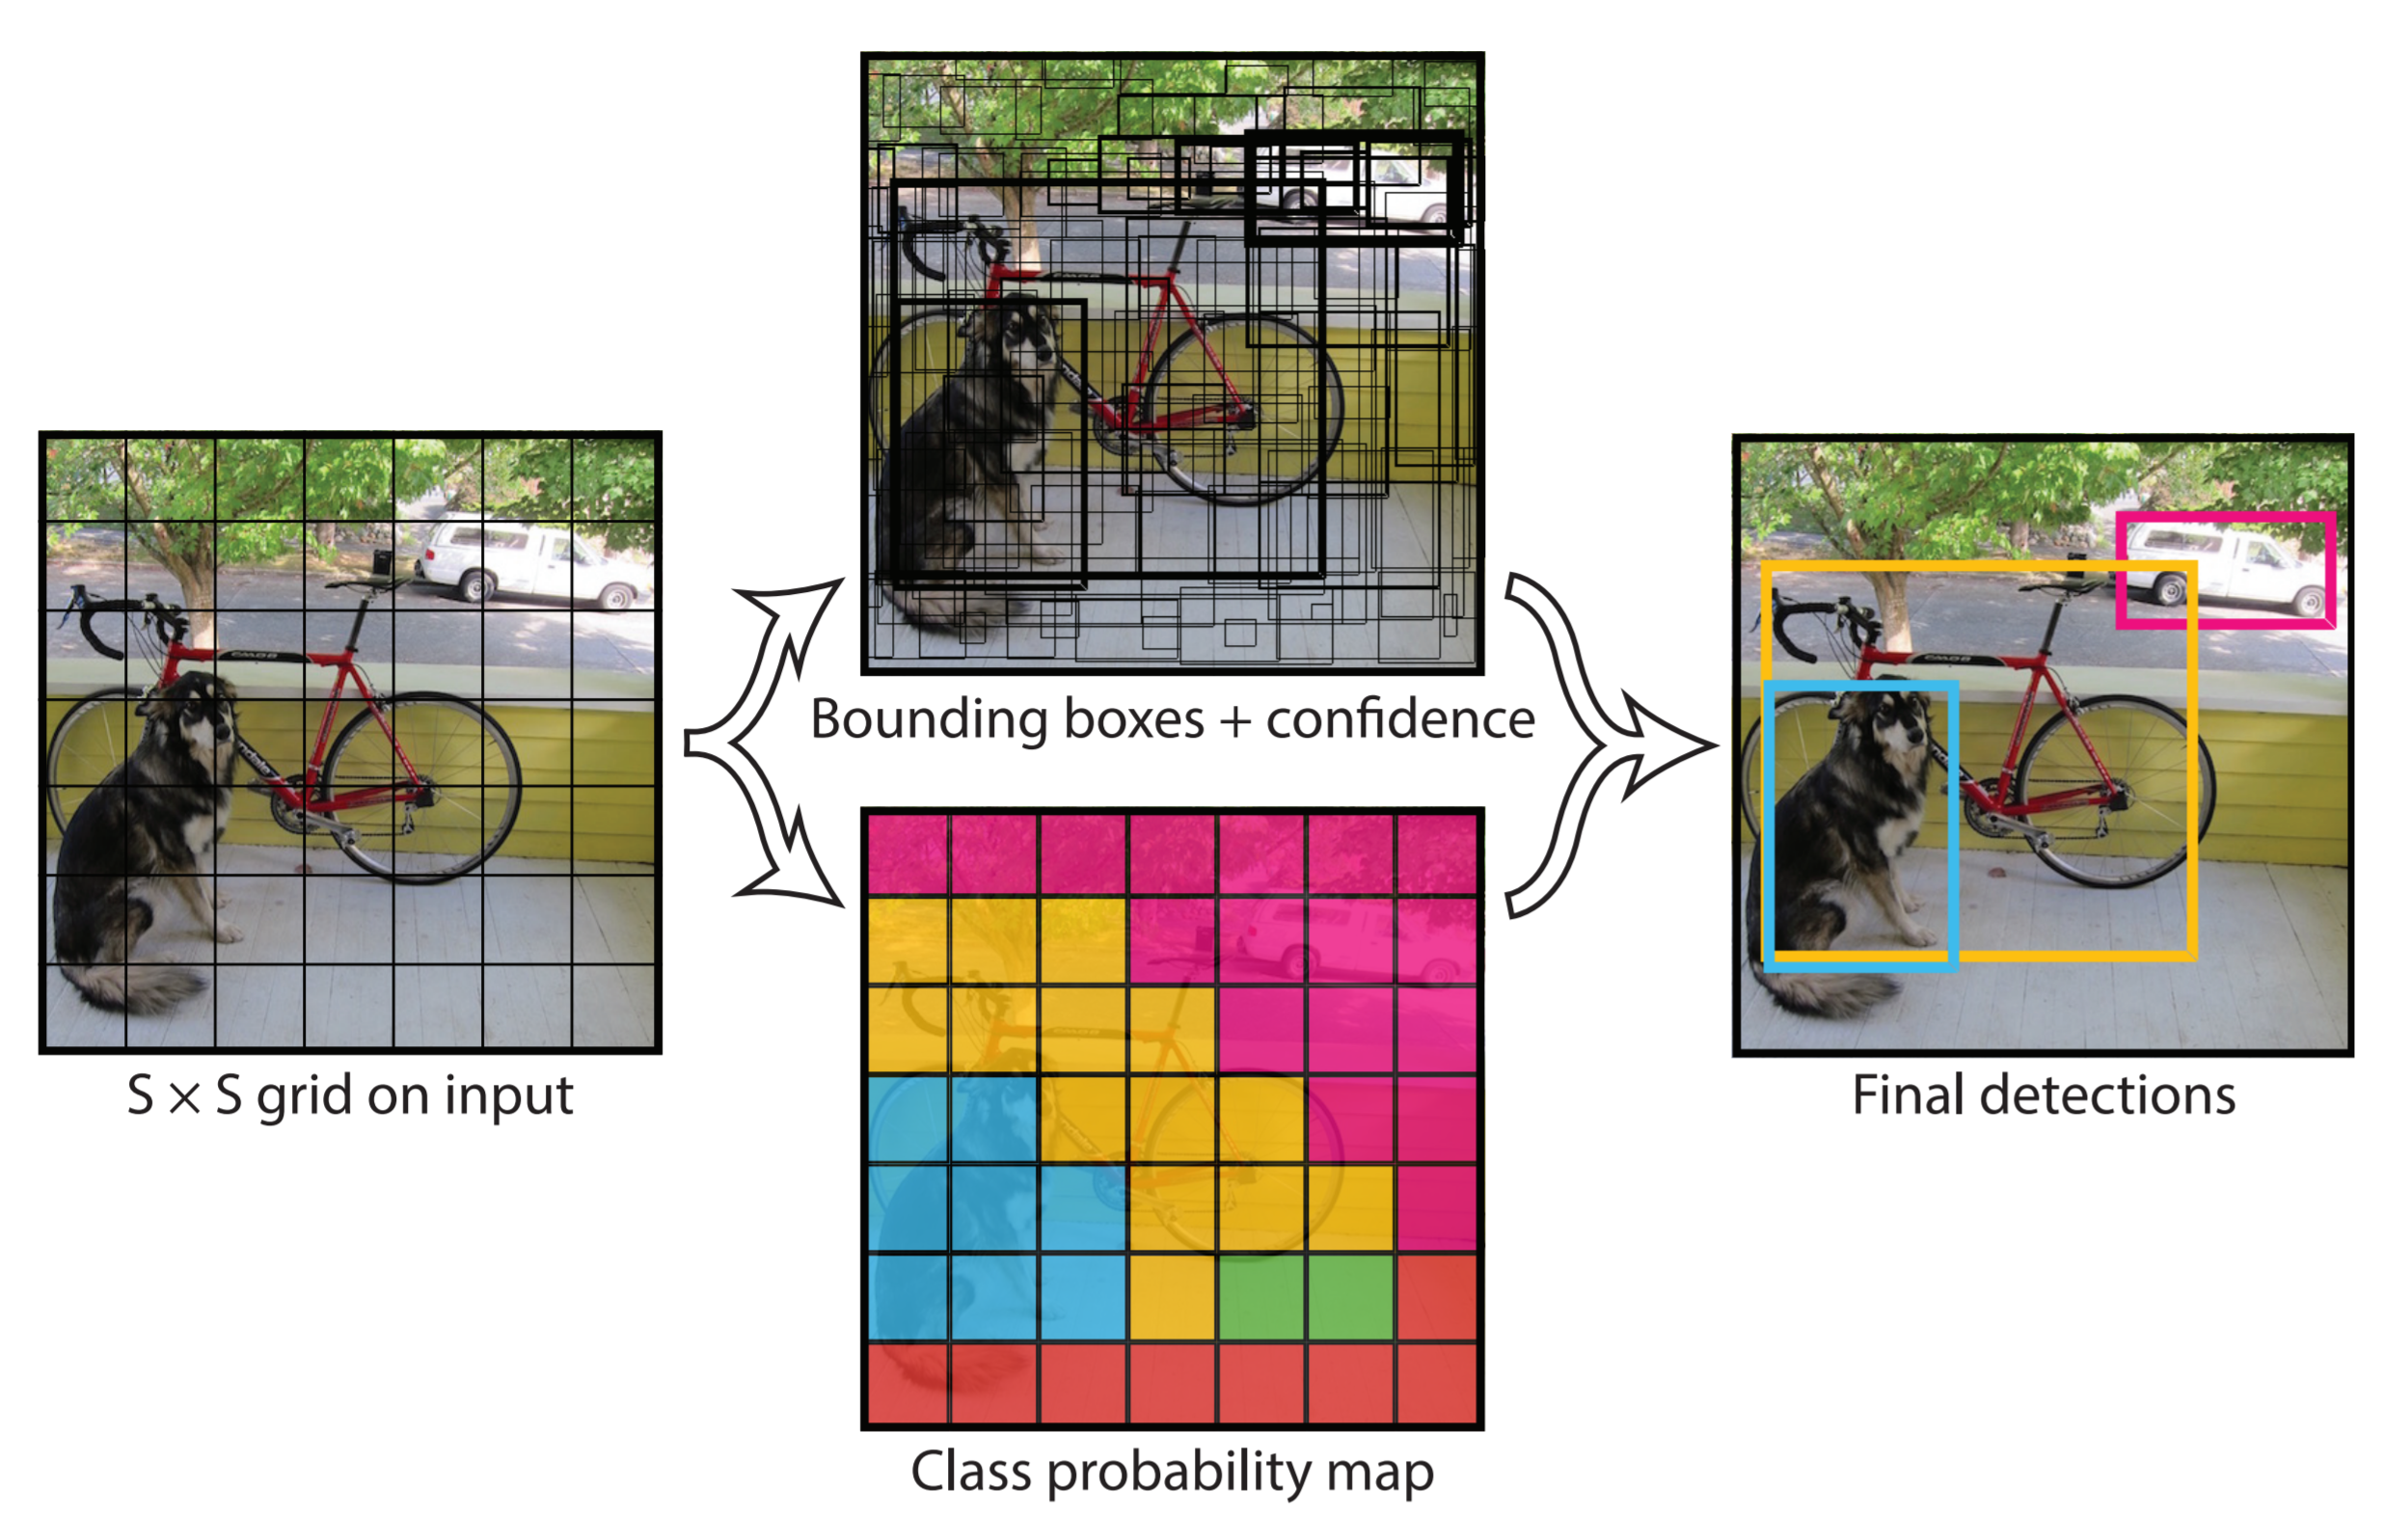
\includegraphics[width=\linewidth]{fig/yolo.png}
    \caption{Framework of YOLO\protect\footnotemark}
    \label{fig:yolo}
\end{figure}

They first split the image into $S \times S$ grids and assign a confidence score vector of length $C$ describing which class of the object in the grid is more likely to have.
For each grid, the model will generate $B$ bounding box centering the grid, each contain the 4-dimensional spatial description and a confidence score for the box.
Applying non-maximum suppression to all $S \times S \times B$ bounding boxes, we get several accurate detections in the image.
\footnotetext{From \cite{redmon2016you}.}

We use YOLOv3\cite{yolov3} to process the images in the MOT16 dataset to obtain detections, and use the deep feature network in DeepSORT to extract features from those detections.
The result of running tracking based on YOLO detections is shown in Table~\ref{tab:eval-yolo}.

\begin{table}[h]
    \caption{Evaluation Result of Tracking with YOLO}
    \label{tab:eval-yolo}
    \begin{tabular}{ccccccccc}
        \hline
        & MOTA & IDF1 & MT & ML & FP & FN & IDs\\\hline
        MOT16-02 & 10.3\% & 26.1\% & 7 & 29 & 3180 & 12729 & 92\\
        MOT16-04 & 36.9\% & 47.4\% & 10 & 27 & 5886 & 23971 & 140\\
        MOT16-05 & 44.4\% & 62.0\% & 32 & 19 & 1233 & 2482 & 79\\
        MOT16-09 & 46.0\% & 44.9\% & 8 & 2 & 1111 & 1669 & 57\\
        MOT16-10 & 29.0\% & 38.1\% & 9 & 20 & 2045 & 6536 & 162\\
        MOT16-11 & 50.6\% & 53.4\% & 21 & 29 & 1074 & 3419 & 36\\
        MOT16-13 & 17.8\% & 31.5\% & 10 & 55 & 1616 & 7563 & 230\\
        OVERALL & 31.8\% & 43.1\% & 97 & 181 & 16145 & 58369 & 796\\\hline
    \end{tabular}
\end{table}

The performance drops from the one in the baseline.
It is possible that the implementation of YOLOv3 is more suitable for circumstances with less detections results, where the image size is limited.
The video in the MOT16 is captured out-door with lots of objects from different classes, and therefore it seems not a good idea to process the video using YOLOv3.

\subsection{Association LSTM}
The multi-object tracking in video can be considered as a task of process some sequence, which is natural to consider using recurrent neural networks to tackle the problem.
Lu \textit{et al.} \cite{lu2017online} implements an association LSTM which refines the detection and association feature from the time-invariant models.
We will briefly review their idea in this section.

In the traditional SORT algorithm, we will use Kalman filters to update the state of an object in the current frame.
Therefore, we can better match the future state of the object with the predicted one than matching the future state with the current state.
The association LSTM shares the similar idea, which not only refines the state of an object through prediction, but also predict the feature of each object.
More specifically, they let the LSTM to refine the feature extracted by some network, possibly the deep cosine features, by making the features of the same object across frames more similar while those of different objects more different.
The association loss \eqref{eq:assoc-loss} in their optimization goal reveals such objective.
\begin{equation}
    \mathcal{L}_{asso} = \sum_t \sum_{i,j} \theta_{ji}|\phi_{t-1}^i \cdot \phi_t^j|
    \label{eq:assoc-loss}
\end{equation}
where $\tilde{f}_t = \{\phi_t^1, \cdots, \phi_t^N\}$ is the refined feature for $N$ objects at time $t$, and $\theta_{ji} \in 0, 1$ is an indicator, which equals 1 iff. object $i$ at time $t-1$ should be associated with object $j$ at time $t$.
The associated objects is expected to have similar features, i.e., higher inner product values.
The higher loss means better performance.

Figure~\ref{fig:lstm-struct} shows their model's structure.
Beside the association loss, there is another term in the loss function of the LSTM, the regression error.
They refines the states of objects through optimizing this term.

\begin{figure}[h]
    \centering
    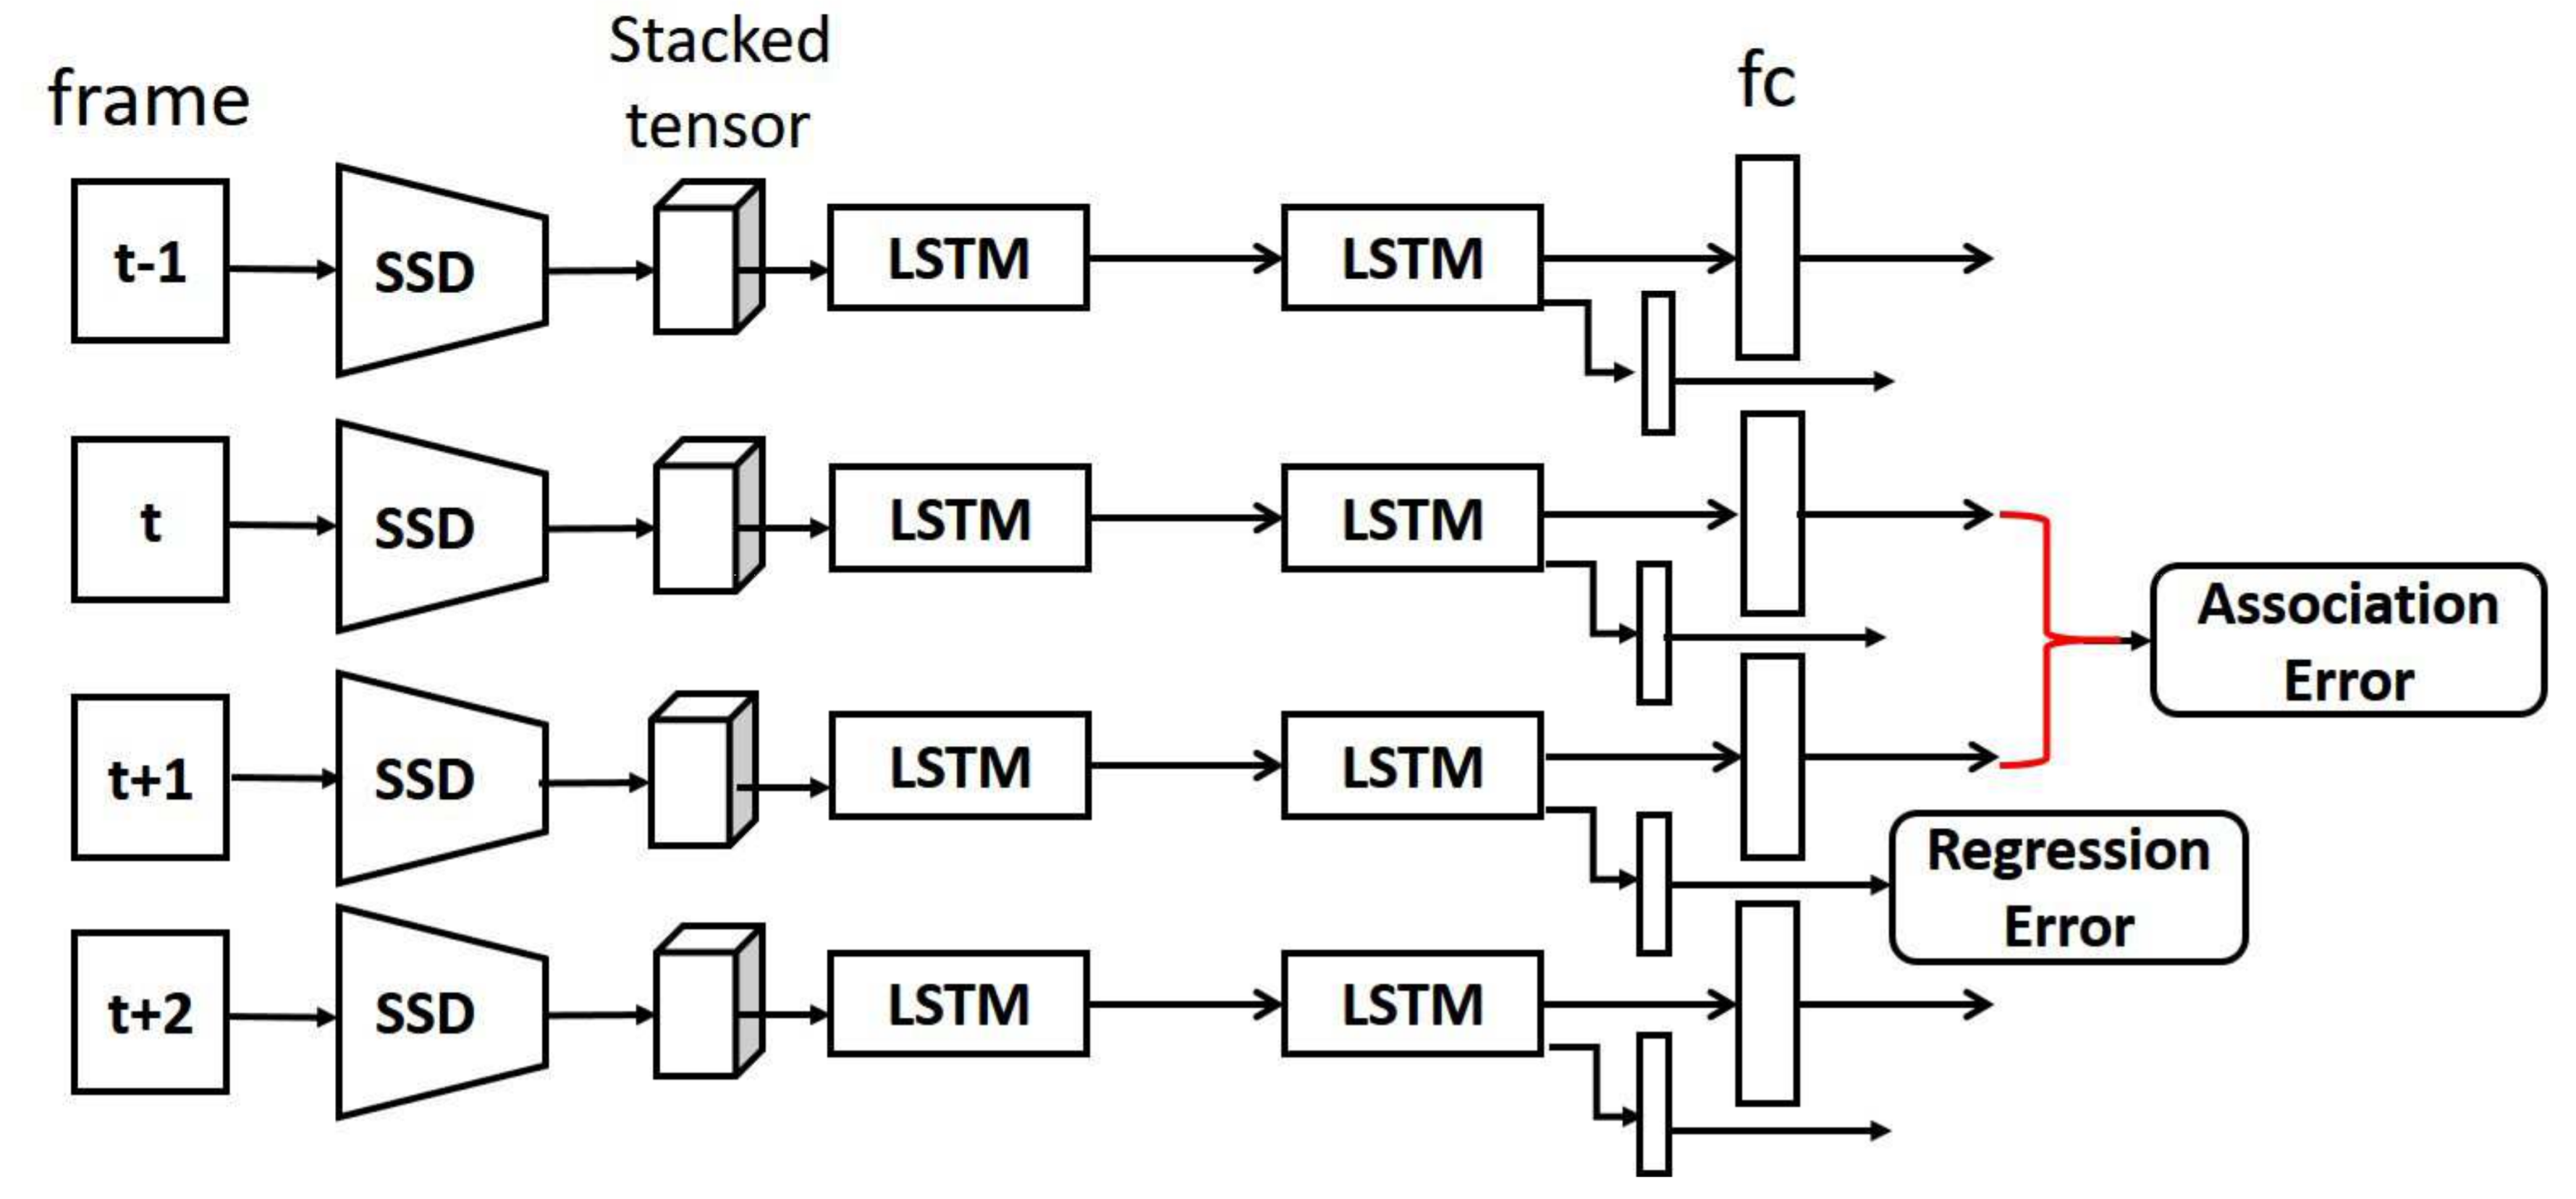
\includegraphics[width=0.99\linewidth]{fig/assoc_lstm.png}
    \caption{Association LSTM Structure\protect\footnotemark}
    \label{fig:lstm-struct}
\end{figure}
\footnotetext{From \cite{lu2017online}.}

As explained before, the functionality of the LSTM layer is similar to the Kalman filter.
However, the advantage of using LSTM is that it stores more information than the Kalman filter, which possesses only the knowledge of the previous frame due to the Markov assumption.
Every frame from the begin to the current one has their influences on the output of the LSTM at the current time stamp, allowing the network to fully utilize the information of the previous video.

We attempt to find some existing code implementing the idea but failed to do so.
We also try to implement the association LSTM ourselves but ended up with not enough computational resources to run experiments.
However, we are enlightened by the idea of carrying more information and predicting the transformation of features.
And we propose using Kalman filters to do the both in \cref{sec:our-work}.

\subsection{Deep Hungarian Network}
We have discussed how to upgrade the detection and feature extraction part so far, and now we move on to upgrade the matching algorithm.
The traditional approach is to formulate the problem as a bi-partite matching, where we need to matching objects in the previous frame with those in the current frame to minimizing the total distance (assuming the same object will not transform too much in both the spatial state and feature space), given the distance matrix.
The problem can be solved efficiently with Hungarian algorithm, the input and output of which are both matrices.
Xu \cite{xu2019deepmot} models the algorithm as a deep neural network, where more information and more complex computation can be performed to obtain the matching matrix.

\begin{figure*}
    \centering
    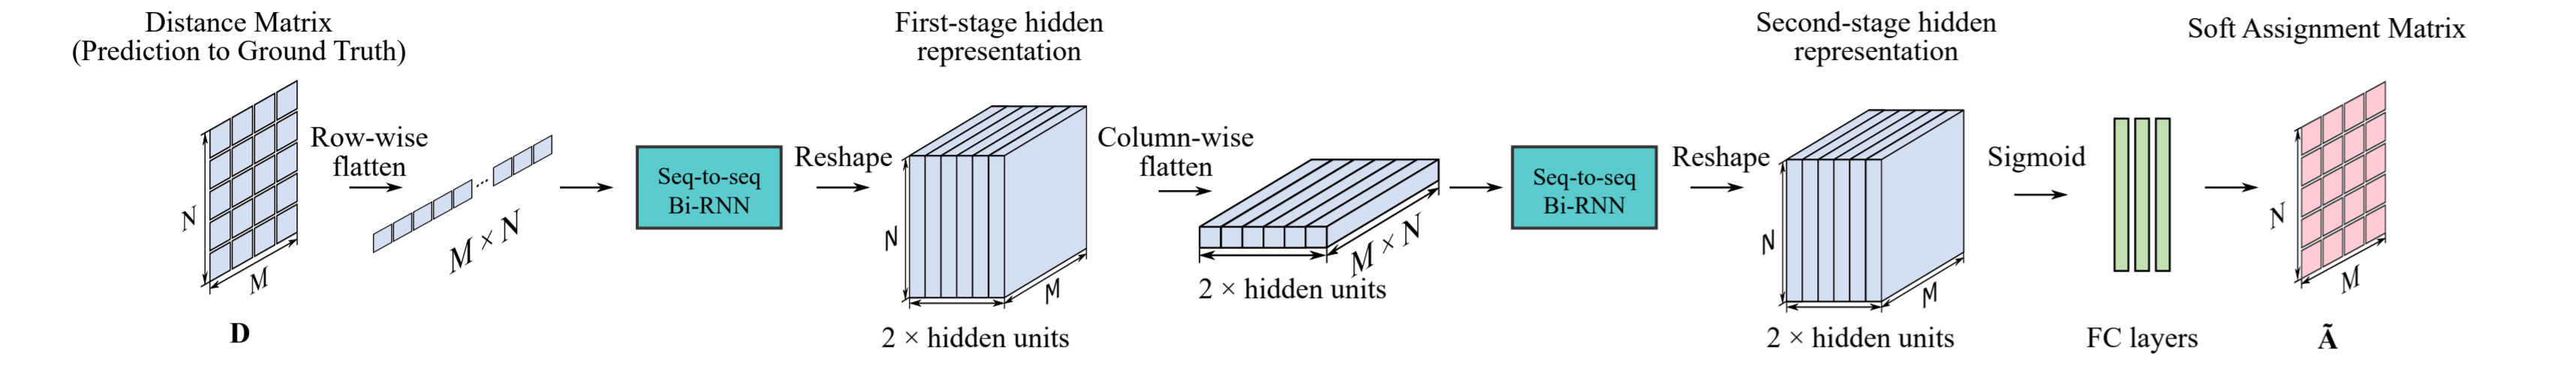
\includegraphics[width=\linewidth]{fig/dhn.png}
    \caption{The Structure of Deep Hungarian Network\protect\footnotemark}
    \label{fig:dhn-struct}
\end{figure*}

The structure of the deep Hungarian network they propose is shown in Figure~\ref{fig:dhn-struct}.
The input distance matrix is first flattened row-wise and processed by a bidirectional recurrent neural network to obtain a set of hidden feature representations.
After flatten the representations column-wise, they are then processed by another recurrent layer and some fully connected layers to obtain the soft assignment matrix.
The row-wise and column-wise flatten operations are to simulate the original Hungarian algorithm.

\footnotetext{From \cite{xu2019deepmot}.}

We had planned to integrate the refined feature matrix obtained from the association LSTM with the DHN, because the fixed output feature size is perfect for the input to the DHN.
But the failure to re-implement the former one causes us unable to try out such combination.
We run the code come along with the paper to get tracking performance on the training set of MOT16 and obtain Table~\ref{tab:eval-deepmot}.

\linespread{1.2}
\begin{table}[h]
    \caption{Evaluation Result of DeepMOT}
    \label{tab:eval-deepmot}
    \begin{tabular}{ccccccccc}
        \hline
        & MOTA & IDF1 & MT & ML & FP & FN & IDs\\\hline
        MOT16-02 & 21.5\% & 30.9\% & 6 & 25 & 1688 & 12240 & 77\\
        MOT16-04 & 15.7\% & 40.5\% & 11 & 28 & 16470 & 23435 & 166\\
        MOT16-05 & 15.8\% & 27.9\% & 3 & 88 & 677 & 5013 & 49\\
        MOT16-09 & 11.1\% & 41.4\% & 9 & 3 & 2788 & 1822 & 63\\
        MOT16-10 & 26.8\% & 40.5\% & 9 & 24 & 2243 & 6716 & 56\\
        MOT16-11 & 39.1\% & 47.4\% & 14 & 31 & 1826 & 3729 & 30\\
        MOT16-13 & 11.5\% & 30.6\% & 7 & 70 & 1279 & 8827 & 23\\
        OVERALL & 19.2\% & 38.4\% & 59 & 269 & 26971 & 61782 & 464\\\hline
    \end{tabular}
\end{table}
\linespread{1.0}

Compared to the deep SORT, the MOTA drops dramatically with lots of false positive and false negative increase.
The index switch count decreases, which could be caused due to the decrease of successful trackings, and therefore this index does not hold much meaning.
The DeepMOT treats the matching problem as a black box, which allows more advanced techniques like DNN to take effect, while giving up the strong prior knowledge of how to solve it.
This trade-off is not very economical, which might be the cause for the performance drop of such method.

% The deep Hungarian network has many problems.
% It is a black box algorithm, whereas the Hungarian algorithm is a white box one and is proved to be reasonable.
% It is believed that 

\section{Our Work: Integrated Real Time Tracking Application}
Next, we implement a real-time tracking application using the Deep SORT framework.
We use YOLO to generate bounding box detections, and use the deep cosine feature extractor to generate features for those bounding boxes.
We use the interface in the Deep SORT code to perform the matching and visualize the trackers.

\section{Our Work: Using More Kalman Filters}
\label{sec:our-work}
\subsection{Extended State Space}

Extending the state vector is a natural idea. A state space of higher dimensions should be able to characterize the state of object in video with more precision. The constant velocity model proposed by \cite{Wojke2017simple}, where the position, aspect ratio and height of a track changes linearly over time, is simple and should apply to most pedestrians, but fail to account for some complex cases, such as the one shown in Fig.~\ref{fig:example-of-nonlinearity}. Therefore, we augment the state space first with acceleration (2nd order) using the constant acceleration model and later higher order terms.

\begin{figure}[h]
    \centering
    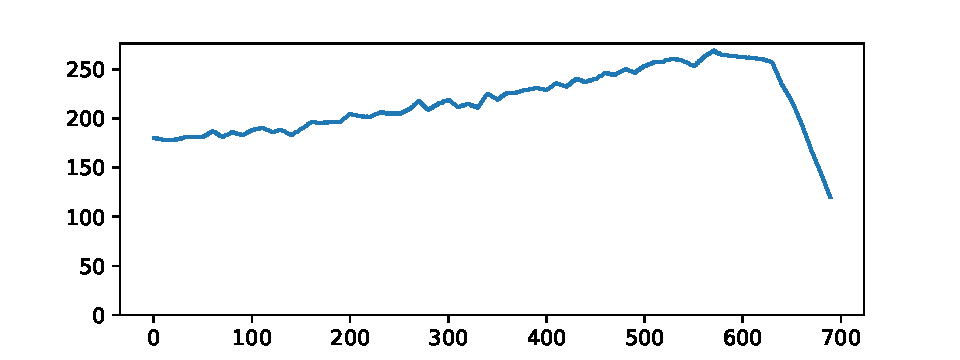
\includegraphics[width=\linewidth]{fig/accelerating-pedestrian-height-plot.pdf}
    \caption{An example of the nonlinear behavior of a state variable. The height of the pedestrian 70 in the sequence MOT16-02 is plotted against time. The pedestrian first moves towards camera and then exits the field of view.}
    \label{fig:example-of-nonlinearity}
\end{figure}

We give an example of augmenting the state space with acceleration below. The new state vector is
\[
    s = [x, y, a, h, v_x, v_y, v_a, v_h, a_x, a_y, a_a, a_h].
\]

Using the example of $x$-coordinate, the state-transition equation is
\[
    x_{k + 1} = x_k + v_{xk} \Delta t + \frac{1}{2} a_{xk} \Delta t^2.
\]

For the velocity, the equation is
\[
    v_{x, k + 1} = v_{xk} + a_{xk} \Delta t.
\]

The equations for other state variables are similar. The state-transition equation for the state vector is
\[
    s_{k + 1} = Fs_k + w_k,
\]
where $F$ is the new state-transition matrix
\[
    F = \begin{bmatrix}
        I_4 & \Delta t I_4 & \frac{1}{2} \Delta t^2 I_4\\
        \mathcal{O} & I_4 & \Delta t I_4\\
        \mathcal{O} & \mathcal{O} & I_4
    \end{bmatrix}
\]
and $w_k$ is noise.

The measurement matrix is
\[
    H = [I_4, \mathcal{O}, \mathcal{O}].
\]

In a similar fashion, the state vector with constant $k$-order terms is a $4(k + 1)$-dimensional vector. The state-transition matrix is $4(k + 1) \times 4(k + 1)$ and the measurement matrix $4 \times 4(k + 1)$ in this case.

To implement the Kalman filter with extended state space, we modified the file \texttt{kalman\_filter.py} to extend the state vector and replace the measurement matrix and the state-transition matrix. We obtain minor improvements over baseline with the addition of acceleration, as shown in Table~\ref{tab:extended-state-space}. With a 0.1\% drop in MOTA, we observe noticeable improvements in the metric IDF1, IDP and IDR (IDP and IDR not shown in the table, but their improvements are comparable to that of IDF1).

Our implementation of the extended state space is flexible enough that constant terms of arbitrary order can be added to the state space. Therefore, we further experiment with 3rd- and 4th-order terms in the state vector. Our experiments have shown that adding more higher-order terms has an adverse effect on the tracking performance. As an example, adding 3rd-order terms showed degraded performance in every metric that we have measured. The following two factors are unfavorable to adding more higher-order terms:

\begin{itemize}
    \item Floating-point operations start to overflow/underflow \emph{consistently} at 4th-order terms in the covariance matrix, in our experiments. Since the covariance matrix is an indication of uncertainty, our initial guess is that there is simply too much uncertainty in higher-order terms.
    \item Because only zeroth-order terms are measured, it is inherently difficult to estimate higher-order terms.
\end{itemize}

\linespread{1.2}
\begin{table}
    \caption{Evaluation result of extended state space (acceleration only)}
    \label{tab:extended-state-space}
    \begin{tabular}{ccccccccc}
        \hline
         & MOTA & IDF1 & MT & ML & FP & FN & IDs\\
        \hline
        MOT16-02 & 33.8\% & 43.4\% & 8 & 12 & 2547 & 9158 & 93\\
        MOT16-13 & 60.3\% & 62.1\% & 52 & 9 & 1523 & 2801 & 217\\
        MOT16-09 & 64.9\% & 62.4\% & 12 & 1 & 191 & 1630 & 25\\
        MOT16-11 & 68.1\% & 64.5\% & 23 & 12 & 426 & 2467 & 37\\
        MOT16-05 & 52.9\% & 58.5\% & 25 & 27 & 451 & 2701 & 58\\
        MOT16-10 & 55.9\% & 62.5\% & 23 & 1 & 1989 & 3322 & 118\\
        MOT16-04 & 58.7\% & 72.0\% & 42 & 18 & 5299 & 14283 & 49\\
        OVERALL & 55.3\% & 63.7\% & 185 & 80 & 12426 & 36362 & 597\\
        \hline
    \end{tabular}
\end{table}
\linespread{1}

\subsection{Filtering on Features}

In this section, we want to apply filtering on latent feature vector extracted by the detector front end. This part is not implemented due to time issues, but regarded as directions worth exploring in the future.

The idea is to apply Kalman Filter directly on the feature vectors extracted by the detector. This requires a few assumptions on the detector and the distribution of the feature vector. One of them is that the feature vectors learned by the detector forms a smooth surface in high dimensional space, and within a small range, it can be treated as linear.  The other is that between two consecutive frames, the feature vector will not change by a large scale and can be modeled by a linear transition equation.

Under these assumptions, we will create a bank of Kalman filters, each with a different transition matrix. When a new frame comes, detections and corresponding features will be extracted and then sent into this unit. For each detection, we will try to filter its feature vector by all filters in the bank and generate a set of proposed feature vectors. The matching will be done on all derived feature vectors and for one detection, only the matching with highest score will be accepted. Afterwards, all filters in the bank will be updated given the matched detection.

One problem of this idea is how to determine the bank of filters. One idea is to train it through statistical methods by ground truth tracks; another is to just parameterize the transition matrices by machine learning models, e.g. neural networks and train them by back propagation. 

\section{Conclusion}

We test Deep SORT's implementation on the MOT16 dataset and our own video. We survey the field of multiple-object tracking and experiment with the idea of using CNN-LSTM for the tracking problem. Due to the lack of computation resources, we are unable to implement the idea. An alternative approach using the deep Hungarian network fails to yield meaningful results, for which we provide our analysis. Based on our understanding of Deep SORT's implementation, we augment the state space used in the Kalman filter to obtain minor improvement over the original implementation and propose feature filtering as future work. We build a real-time multiple-object tracker based on Deep SORT and YOLO, as the original implementation is not completely real-time.

\bibliographystyle{IEEEtran}
\bibliography{Ref}

\end{document}
